\documentclass[9pt]{IEEEtran}

\usepackage[english]{babel}
\usepackage{graphicx}
\usepackage{epstopdf}
\usepackage{fancyhdr}
\usepackage{amsmath}
\usepackage{amsthm}
\usepackage{amssymb}
\usepackage{url}
\usepackage{array}
\usepackage{textcomp}
\usepackage{listings}
\usepackage{hyperref}
\usepackage{xcolor}
\usepackage{colortbl}
\usepackage{float}
\usepackage{gensymb}
\usepackage{longtable}
\usepackage{supertabular}
\usepackage{multicol}

\usepackage[utf8x]{inputenc}

\usepackage[T1]{fontenc}
\usepackage{lmodern}{}
\input{glyphtounicode}
\pdfgentounicode=1

\graphicspath{{./figures/}}
\DeclareGraphicsExtensions{.pdf,.png,.jpg,.eps}

% correct bad hyphenation here
\hyphenation{op-tical net-works semi-conduc-tor trig-gs}

% ============================================================================================

\title{\vspace{0ex}
Kernels}

\author{Marko Medved\vspace{-4.0ex}}

% ============================================================================================

\begin{document}

\maketitle


\section{Part 1}
In this section we implemented the kernelized ridge regression and support vector
regression. Next to the basic Linear kernel we also implemented the Polynomial 
kernel defined as: 
\[
K(\mathbf{x}, \mathbf{x}') = (\mathbf{x}^\top \mathbf{x}' + c)^M
\]
where M is the degree of the polynomial, and c is a constant which was set to 1.
We also implemented the RBF kernel defined as: 
\[
K(\mathbf{x}, \mathbf{x}') = \exp\left(-\frac{\|\mathbf{x} - \mathbf{x}'\|^2}{2\sigma^2}\right)
\]




\subsection{Kernelized ridge regression implementation}

\subsection{Support vector regression implementation}

\subsection{Fitting both methods to the 1-dimensional sine data}




  \begin{figure}[h]
    \centering
    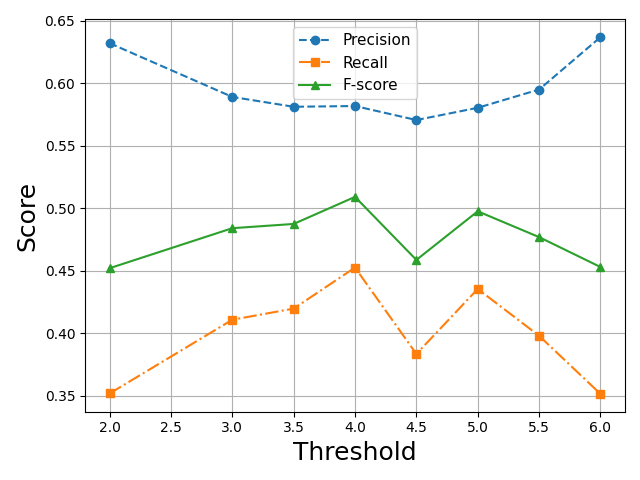
\includegraphics[width=0.99\columnwidth]{figures/thresholds.png}
    \caption{Comparison of performance at different thresholds}
    \label{fig:thresholds}
\end{figure}




\bibliographystyle{IEEEtran}
\bibliography{bibliography}

\end{document}
